\section{Diseño del controlador}

Para controlar la planta a lazo cerrado, se utilizará como modelo base un controlador PID. Este controlador, en tiempo continuo, tiene la siguiente forma
\[
    C(s) = k_p + k_i \frac{1}{s} + k_d s.
\]
En particular, se implmentarán a partir de la expresión anterior un controlador proporcional (tipo P, donde solo $k_p$ es no nulo), proporcional-integral (tipo PI, con $k_d = 0$), y proporcional-derivativo (tipo PD, con $k_i = 0$).

Dado que el controlador será implementado en forma discreta, con $T_s = \qty{20}{\ms}$, se utilizará la siguiente expresión bilineal, donde se reemplaza $s = (z - 1)/(T_s z)$ y se busca una relación de recurrencia en función de la señal error:
\begin{align}
    \label{eq:pid-u}
    u_{k} = k_{p}e_{k} + k_{i}\left(I_{k-1} + \frac{T}{2}e_{k} + \frac{T}{2}e_{k-1}\right) + k_{d}\left(2\frac{e_{k} - e_{k-1}}{T} - D_{k-1}\right),
\end{align}
en donde
\begin{align}
    \label{eq:pid-id}
    I_{k} = I_{k-1} + \frac{T}{2}e_{k} + \frac{T}{2}e_{k-1} && D_{k} = 2\frac{e_{k} - e_{k-1}}{T} - D_{k-1}.
\end{align}

\subsection{Controlador P}

El primer control implementado fue un controlador proporcional, para el cual se aplicaron las Ecuaciones~\eqref{eq:pid-u} y~\eqref{eq:pid-id}, utilizando
\begin{align*}
    K_p = -150, && K_i = 0, && K_d = 0.
\end{align*}

\subsubsection{Rechazo a perturbaciones tipo impulso}

La Figura~\ref{fig:p-pert-salida} muestra la salida de la planta ---la posición del carrito--- real y simulada, ante una perturbación tipo impulso, con el lazo cerrado por el controlador P y una referencia nula (punto de equilibrio).

Se observa que inicialmente hay una concordancia buena entre el modelo y la planta real. Ambos sistemas presentan una oscilación, pero el sistema real se ve severamente afectado por el rozamiento, por lo que llega a estado estacionario tras solo unos segundos. El sistema simulado continúa oscilando durante más tiempo.

\begin{figure}[!htbp]
    \centering
    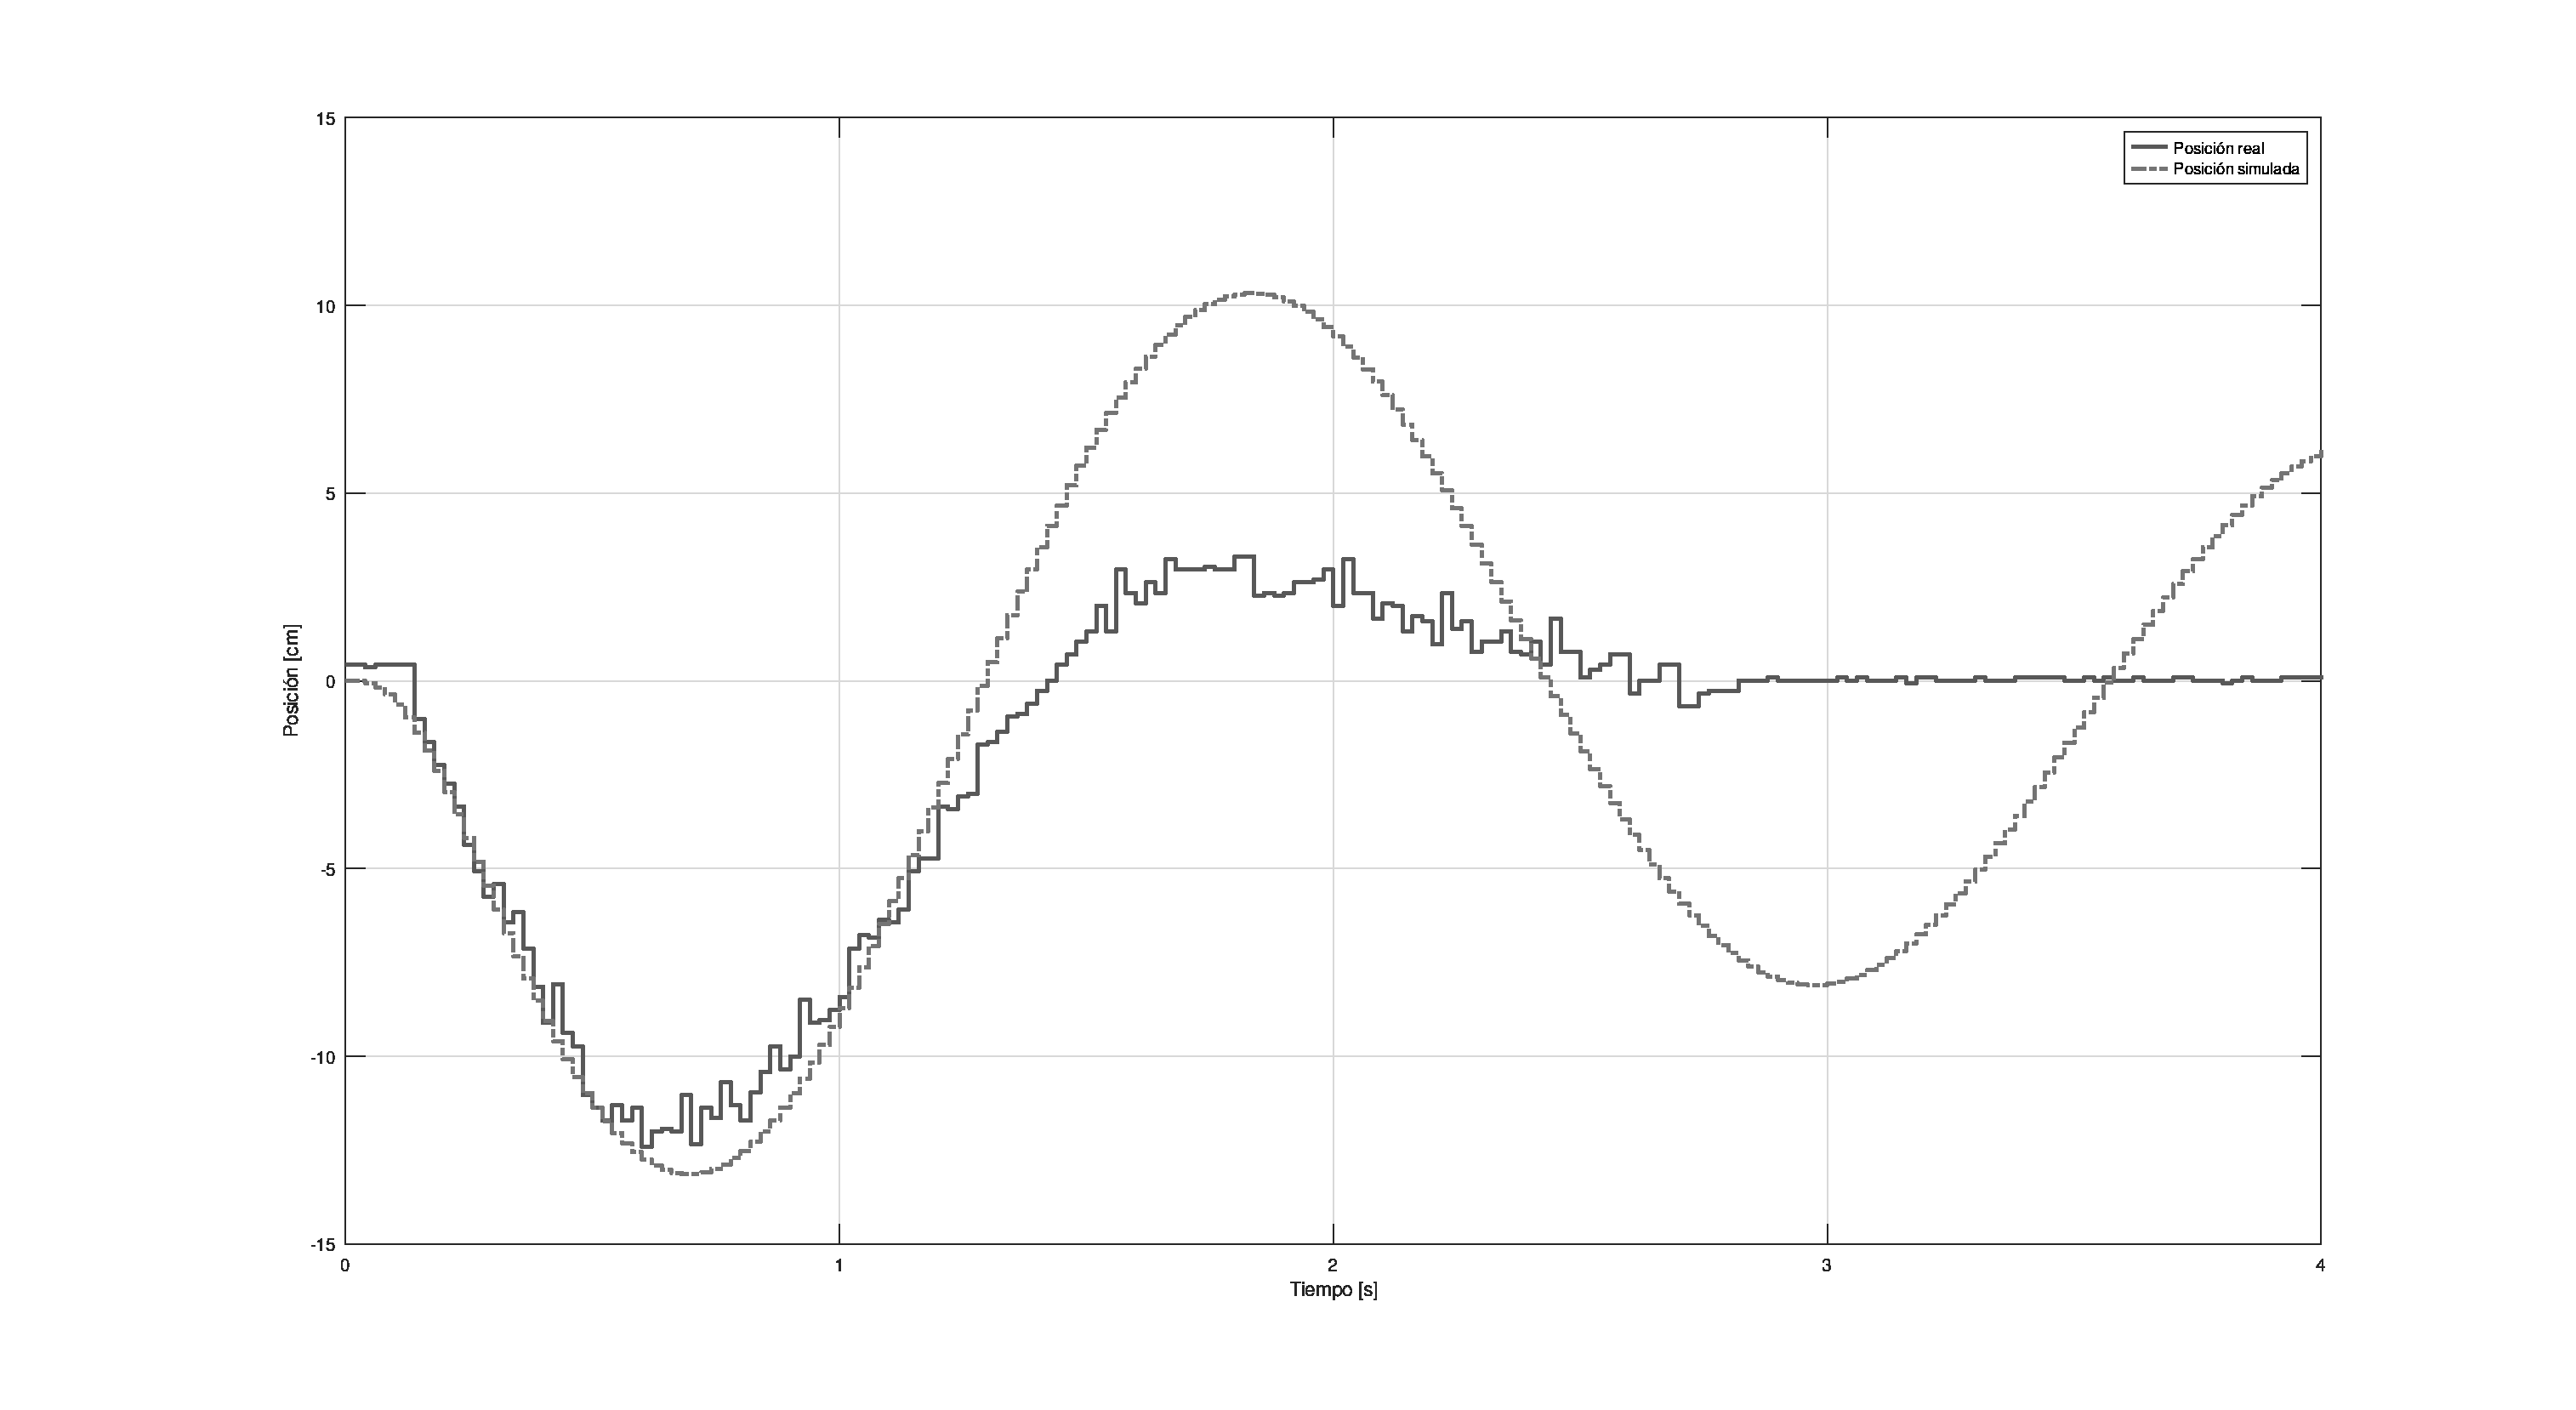
\includegraphics[width=\linewidth]{img/p-pert-salida.eps}
    \caption{Salida del sistema real y simulado ante una perturbación tipo impulso, y un lazo cerrado con un controlador tipo P. Notar que las salidas se escalaron para estar en centímetros.}
    \label{fig:p-pert-salida}
\end{figure}

La Figura~\ref{fig:p-pert-cont} muestra la acción de control ---el comando enviado al servomotor--- real y simulada, ante una perturbación tipo impulso, con el lazo cerrado por el controlador P y una referencia nula (punto de equilibrio). Observar que la acción de control en ningún caso satura los límites impuestos anteriormente. También notar que la forma de onda es la misma que la de la salida (Figura~\ref{fig:p-pert-salida}) salvo un factor de escala, ya que $u = k_p (r - y) = -k_p y$ (y recordar que $k_p < 0$, por lo que $u$ e $y$ tendrán la misma fase).

\begin{figure}[!htbp]
    \centering
    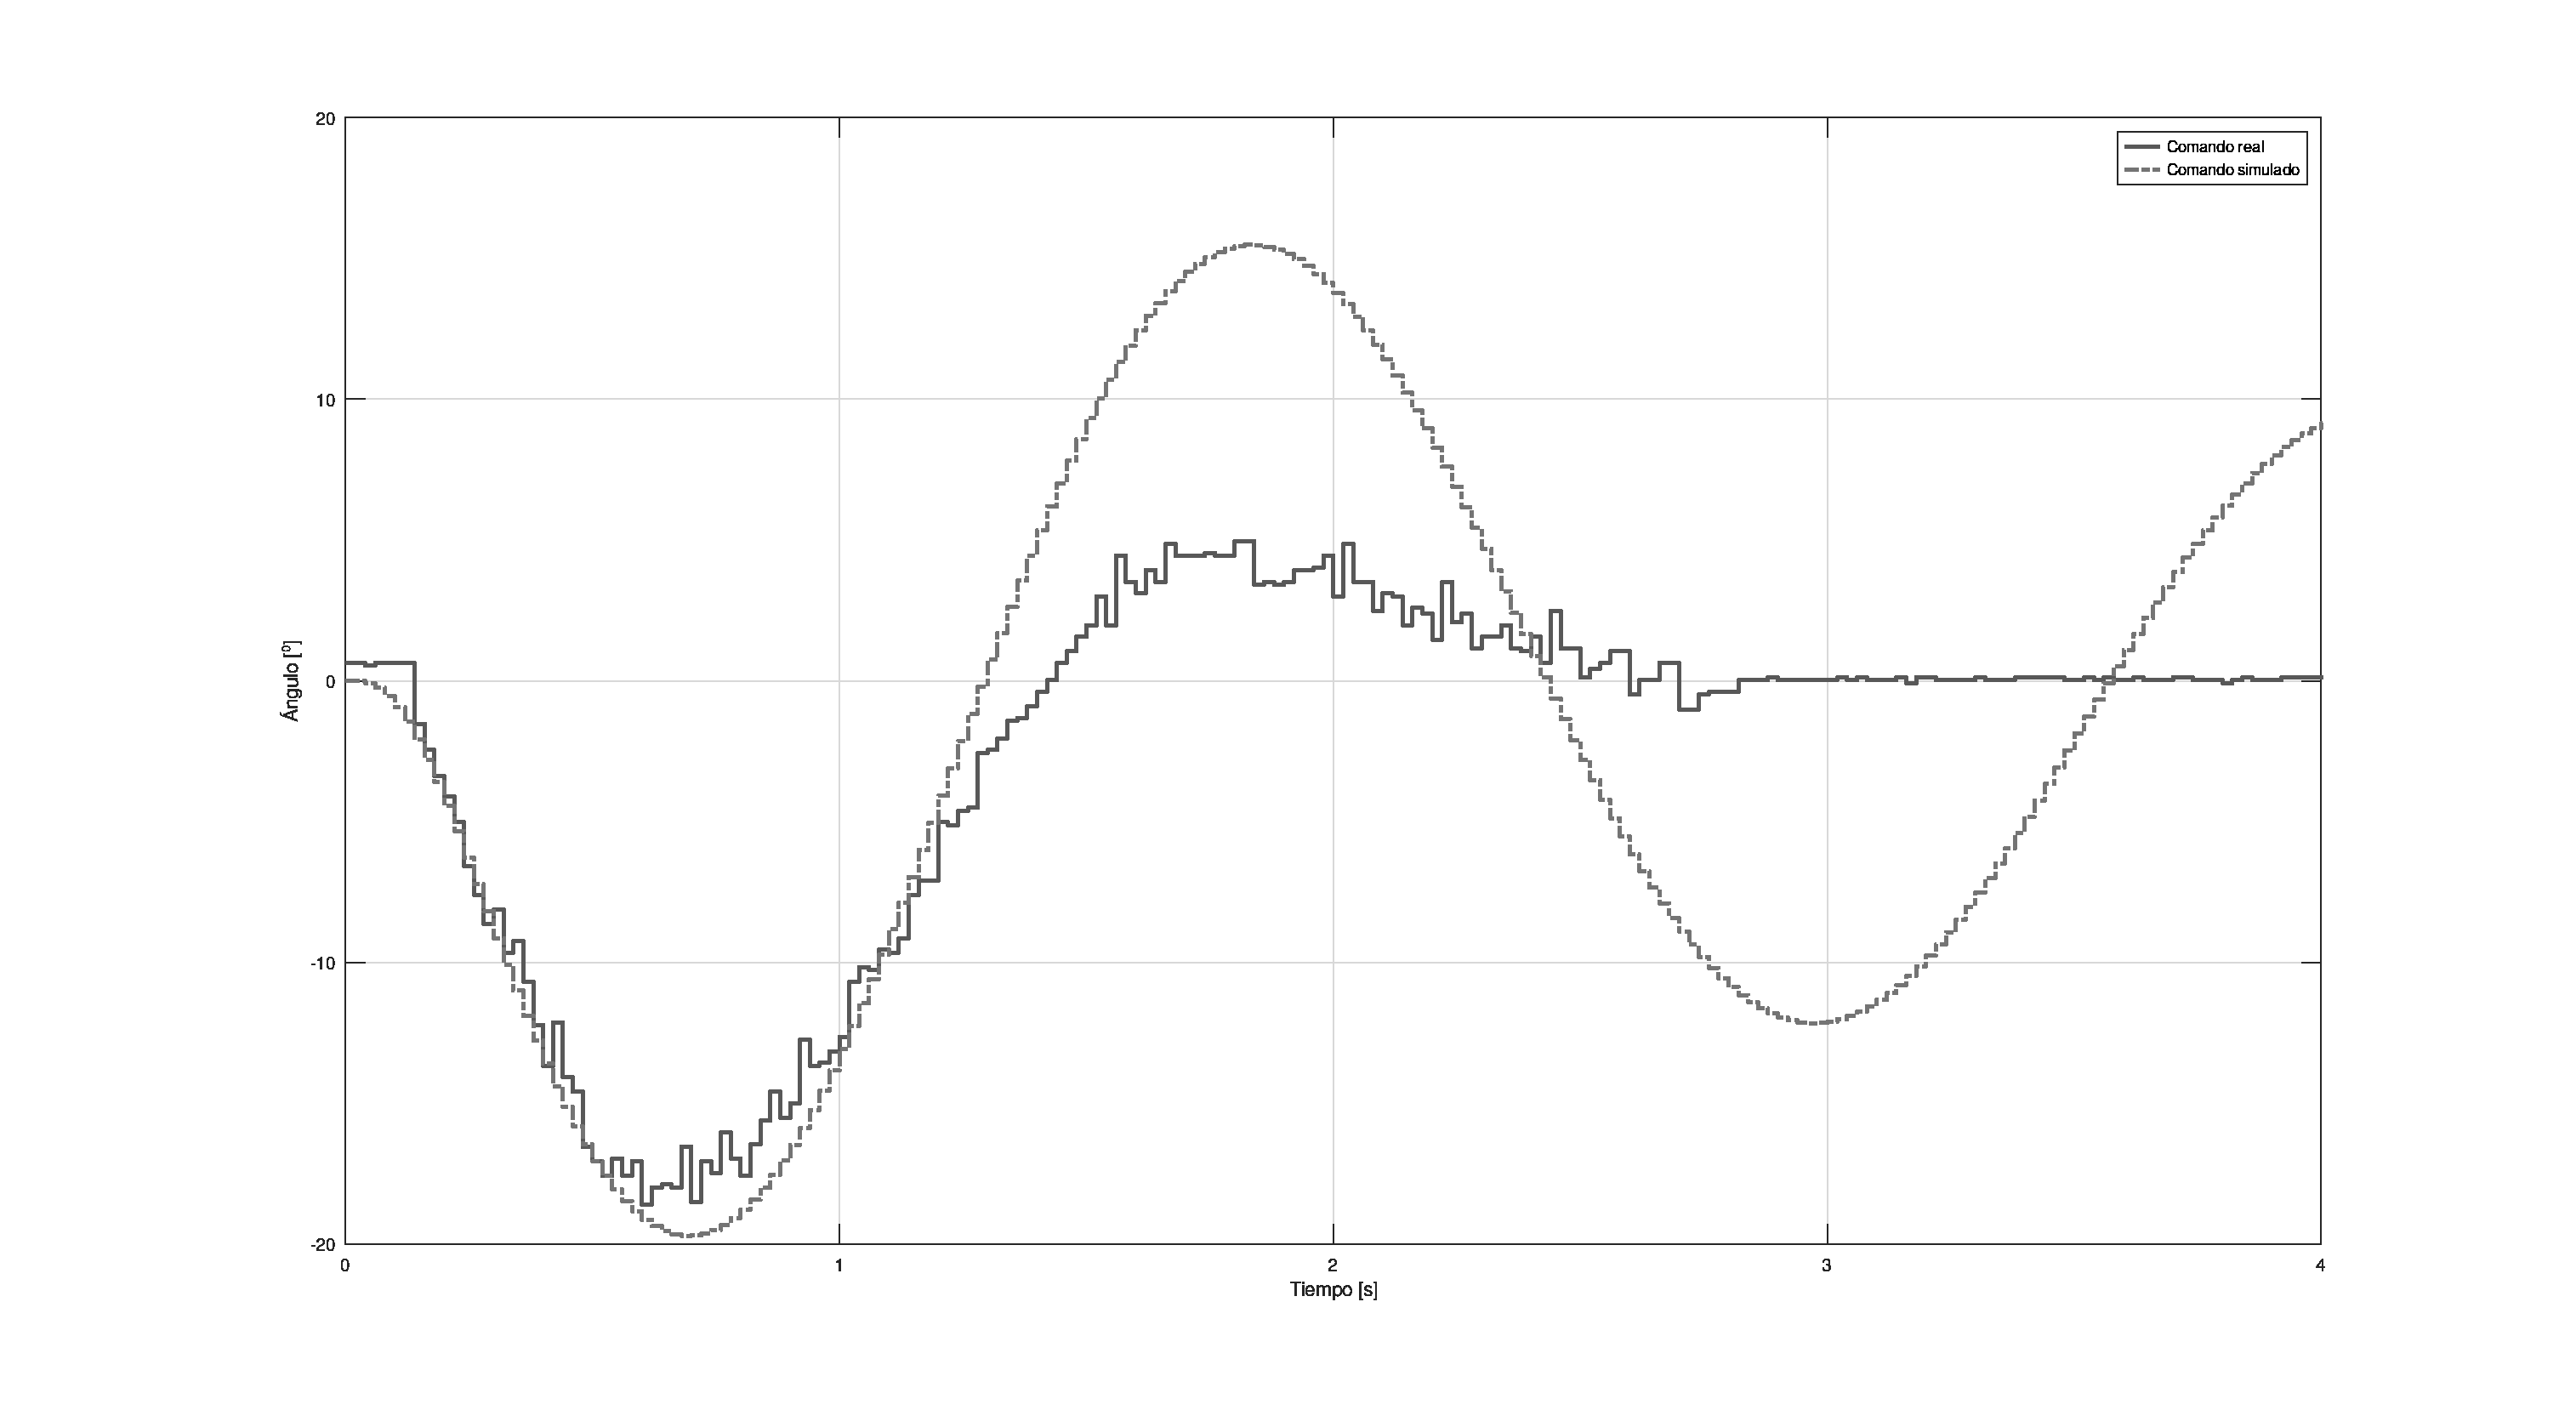
\includegraphics[width=\linewidth]{img/p-pert-cont.eps}
    \caption{Acción de control del sistema real y simulado ante una perturbación tipo impulso, y un lazo cerrado con un controlador tipo P.}
    \label{fig:p-pert-cont}
\end{figure}

\subsubsection{Respuesta al escalón de referencia}

La Figura~\ref{fig:p-ref-salida} muestra la salida de la planta ---la posición del carrito--- real y simulada, ante un escalón de referencia de \qty{0.1}{\m}, con el lazo cerrado por el controlador P.

Por la presencia del integrador en la planta, el controlador simulado eventualmente logra establecer a la planta en la referencia deseada. Sin embargo, producto de la fricción no modelada, el carrito en la realidad se frena. La posición medida no se establece en los \qty{0.1}{\m}, presentando un error no nulo en estado estacionario de aproximadamente un centímetro.

\begin{figure}[!htbp]
    \centering
    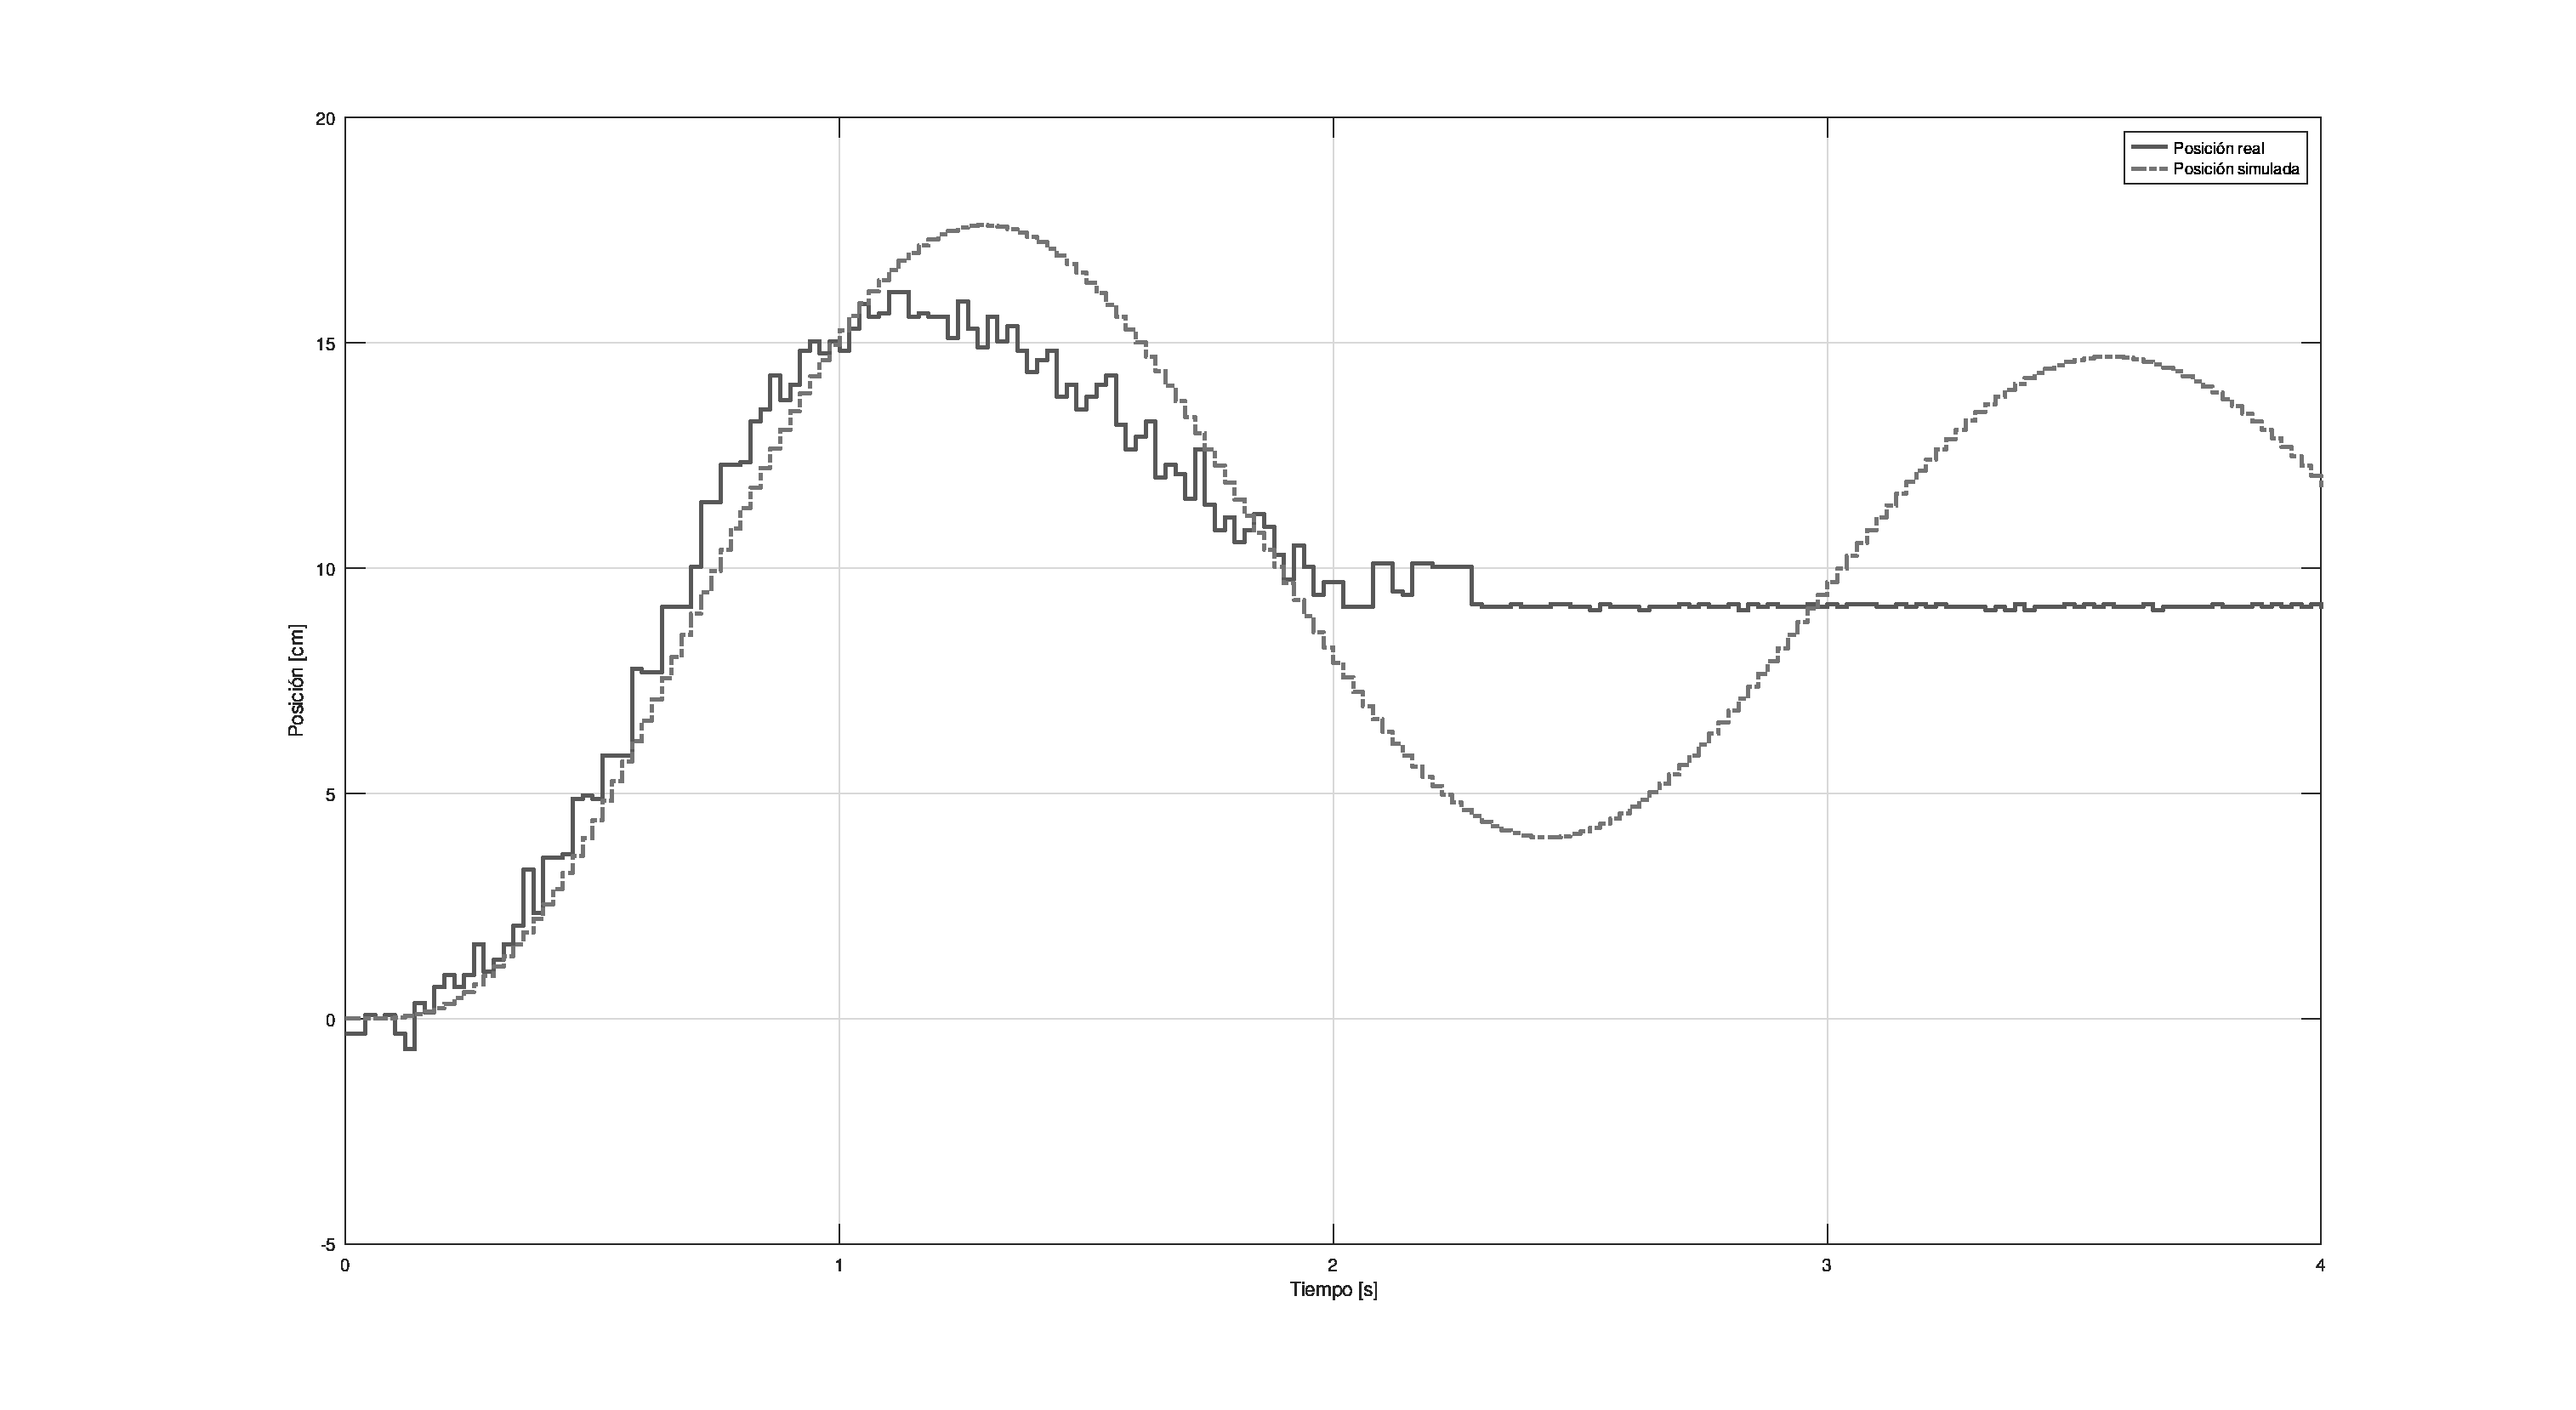
\includegraphics[width=\linewidth]{img/p-ref-salida.eps}
    \caption{Salida del sistema real y simulado ante un escalón de referencia, y un lazo cerrado con un controlador tipo P. Notar que las salidas se escalaron para estar en centímetros.}
    \label{fig:p-ref-salida}
\end{figure}

\subsection{Controlador PI}

El segundo control implementado fue un controlador proporcional-integral, para el cual se aplicaron las Ecuaciones~\eqref{eq:pid-u} y~\eqref{eq:pid-id}, utilizando
\begin{align*}
    K_p = -150, && K_i = -30, && K_d = 0.
\end{align*}

\subsubsection{Rechazo a perturbaciones tipo impulso}

La Figura~\ref{fig:pi-pert-salida} muestra la salida de la planta ---la posición del carrito--- real y simulada, ante una perturbación tipo impulso, con el lazo cerrado por el controlador PI y una referencia nula (punto de equilibrio).

%Se observa que inicialmente hay una concordancia buena entre el modelo y la planta real. Ambos sistemas presentan una oscilación, pero el sistema real se ve severamente afectado por el rozamiento, por lo que llega a estado estacionario tras solo unos segundos. El sistema simulado continúa oscilando durante más tiempo.



\begin{figure}[!htbp]
    \centering
    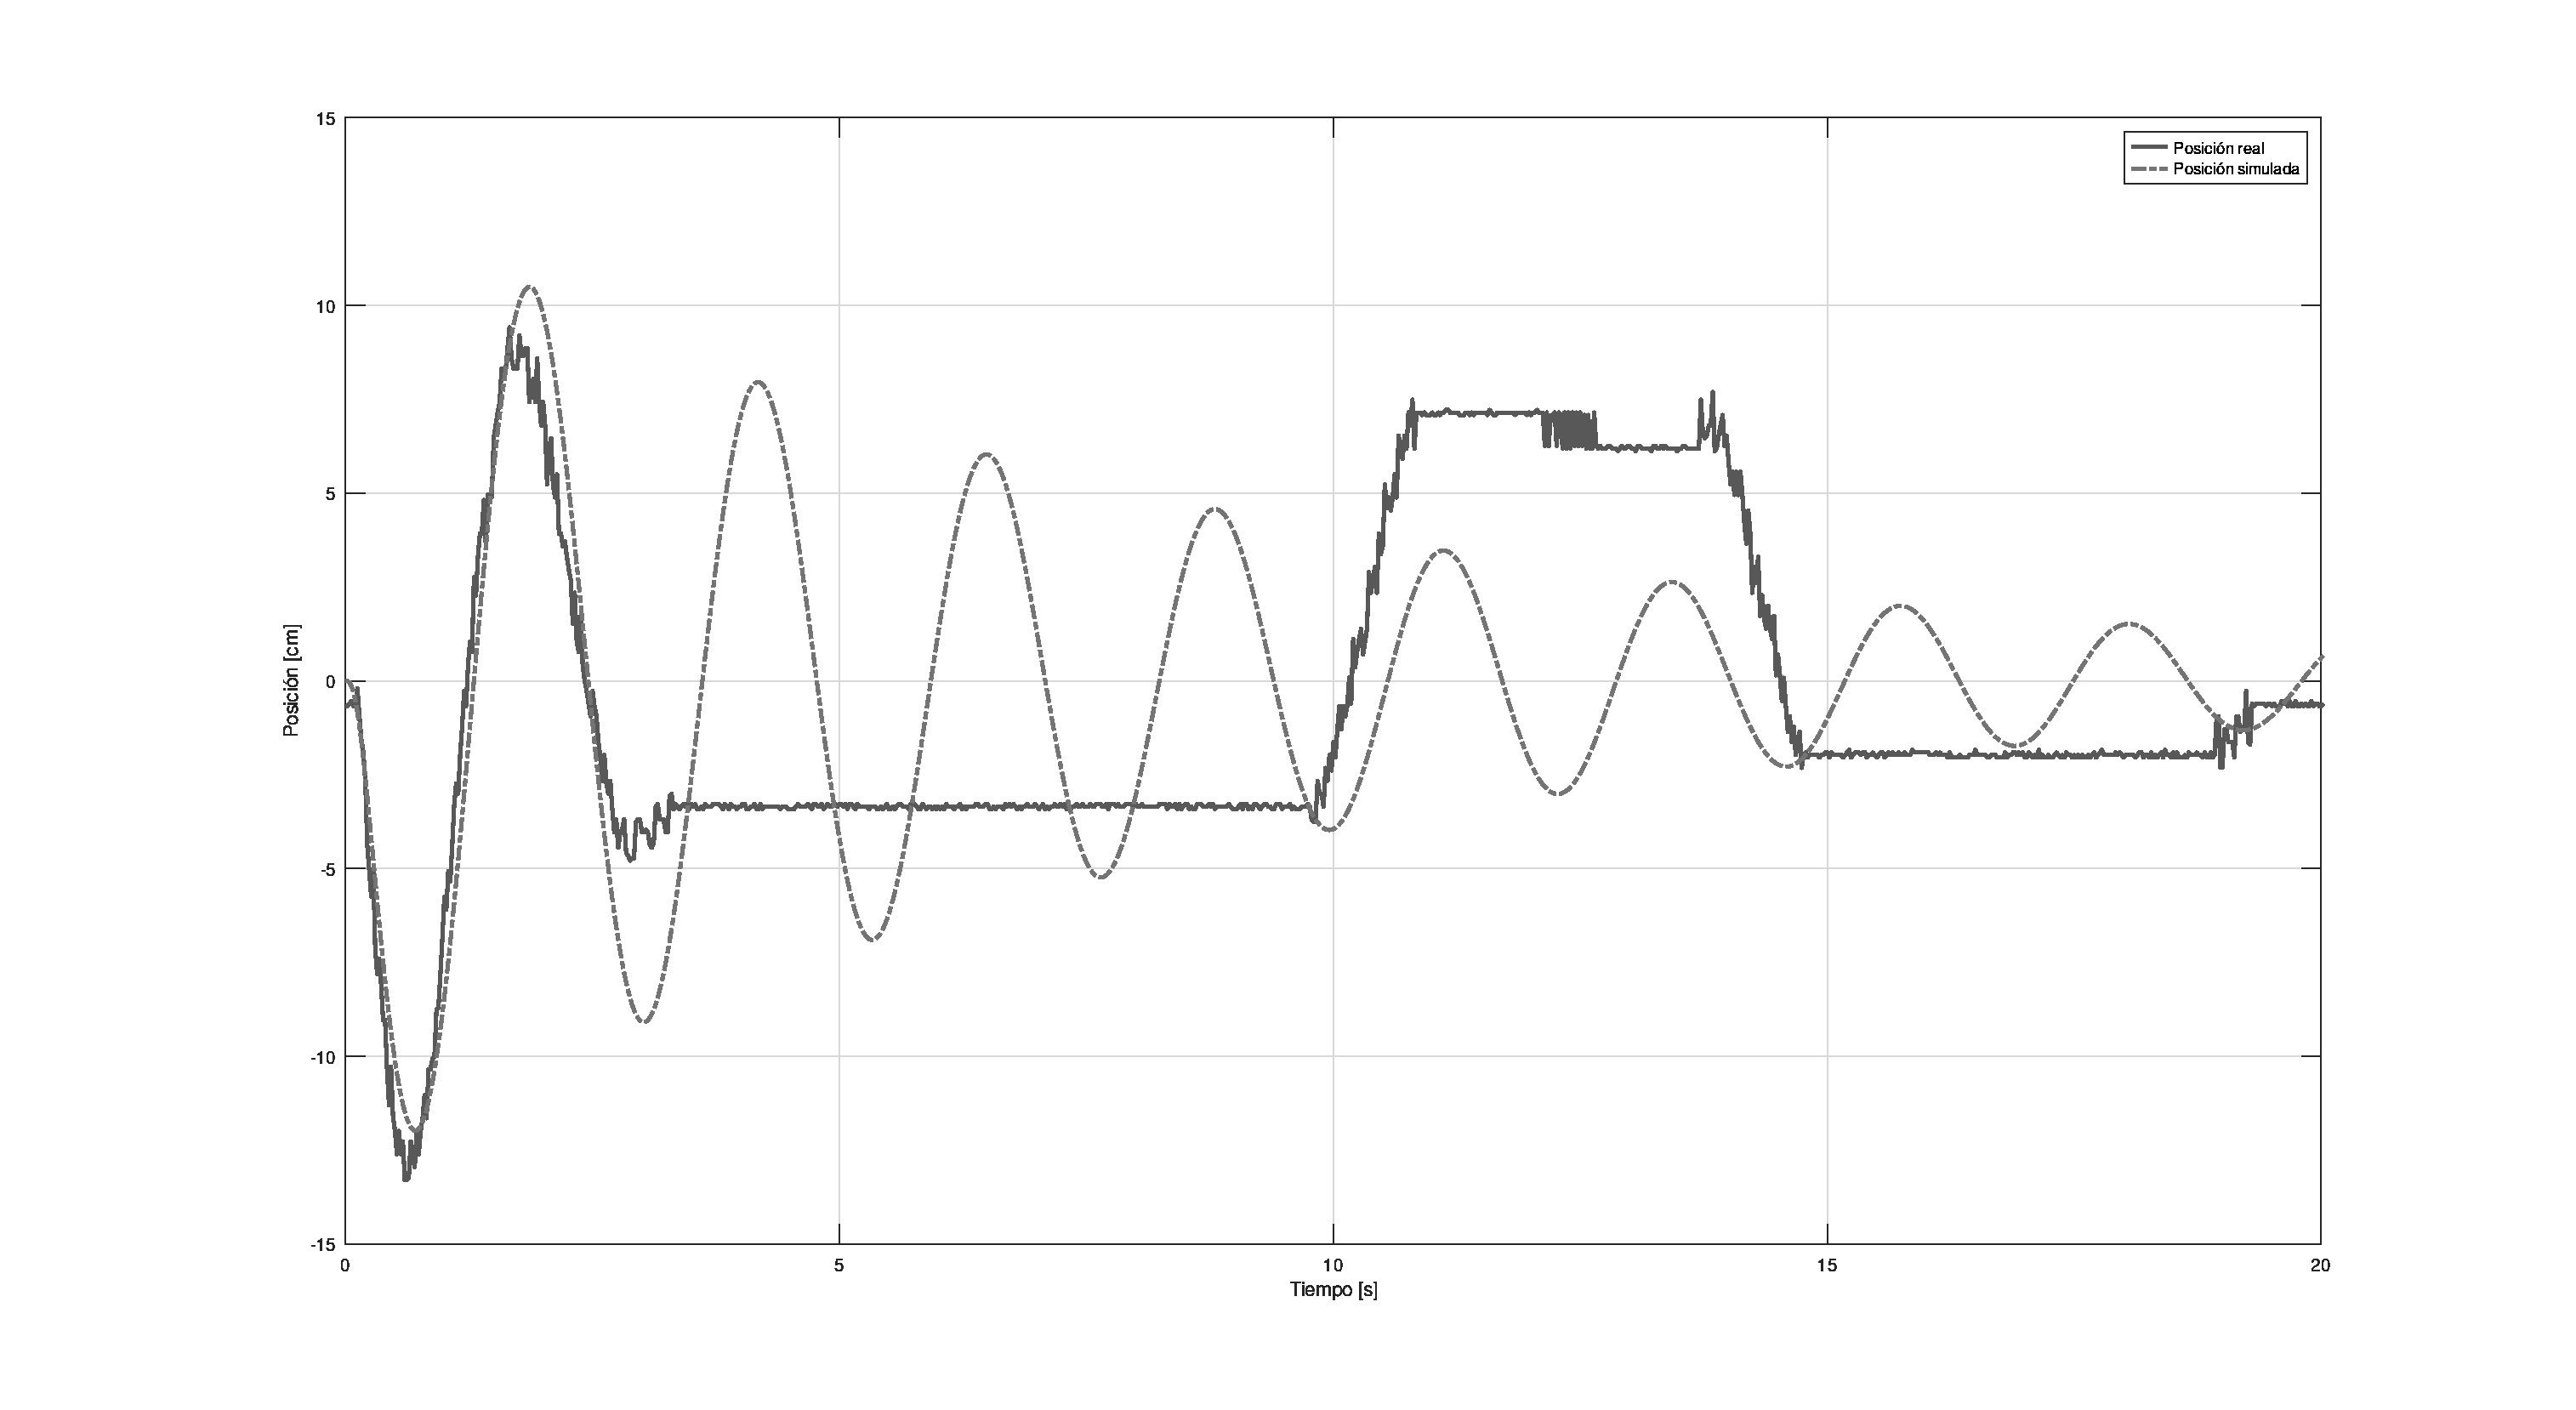
\includegraphics[width=\linewidth]{img/pi-pert-salida.eps}
    \caption{Salida del sistema real y simulado ante una perturbación tipo impulso, y un lazo cerrado con un controlador tipo PI. Notar que las salidas se escalaron para estar en centímetros.}
    \label{fig:pi-pert-salida}
\end{figure}

%La Figura~\ref{fig:p-pert-cont} muestra la acción de control ---el comando enviado al servomotor--- real y simulada, ante una perturbación tipo impulso, con el lazo cerrado por el controlador P y una referencia nula (punto de equilibrio). Observar que la acción de control en ningún caso satura los límites impuestos anteriormente. También notar que la forma de onda es la misma que la de la salida (Figura~\ref{fig:p-pert-salida}) salvo un factor de escala, ya que $u = k_p (r - y) = -k_p y$ (y recordar que $k_p < 0$, por lo que $u$ e $y$ tendrán la misma fase).
%
\begin{figure}[!htbp]
    \centering
    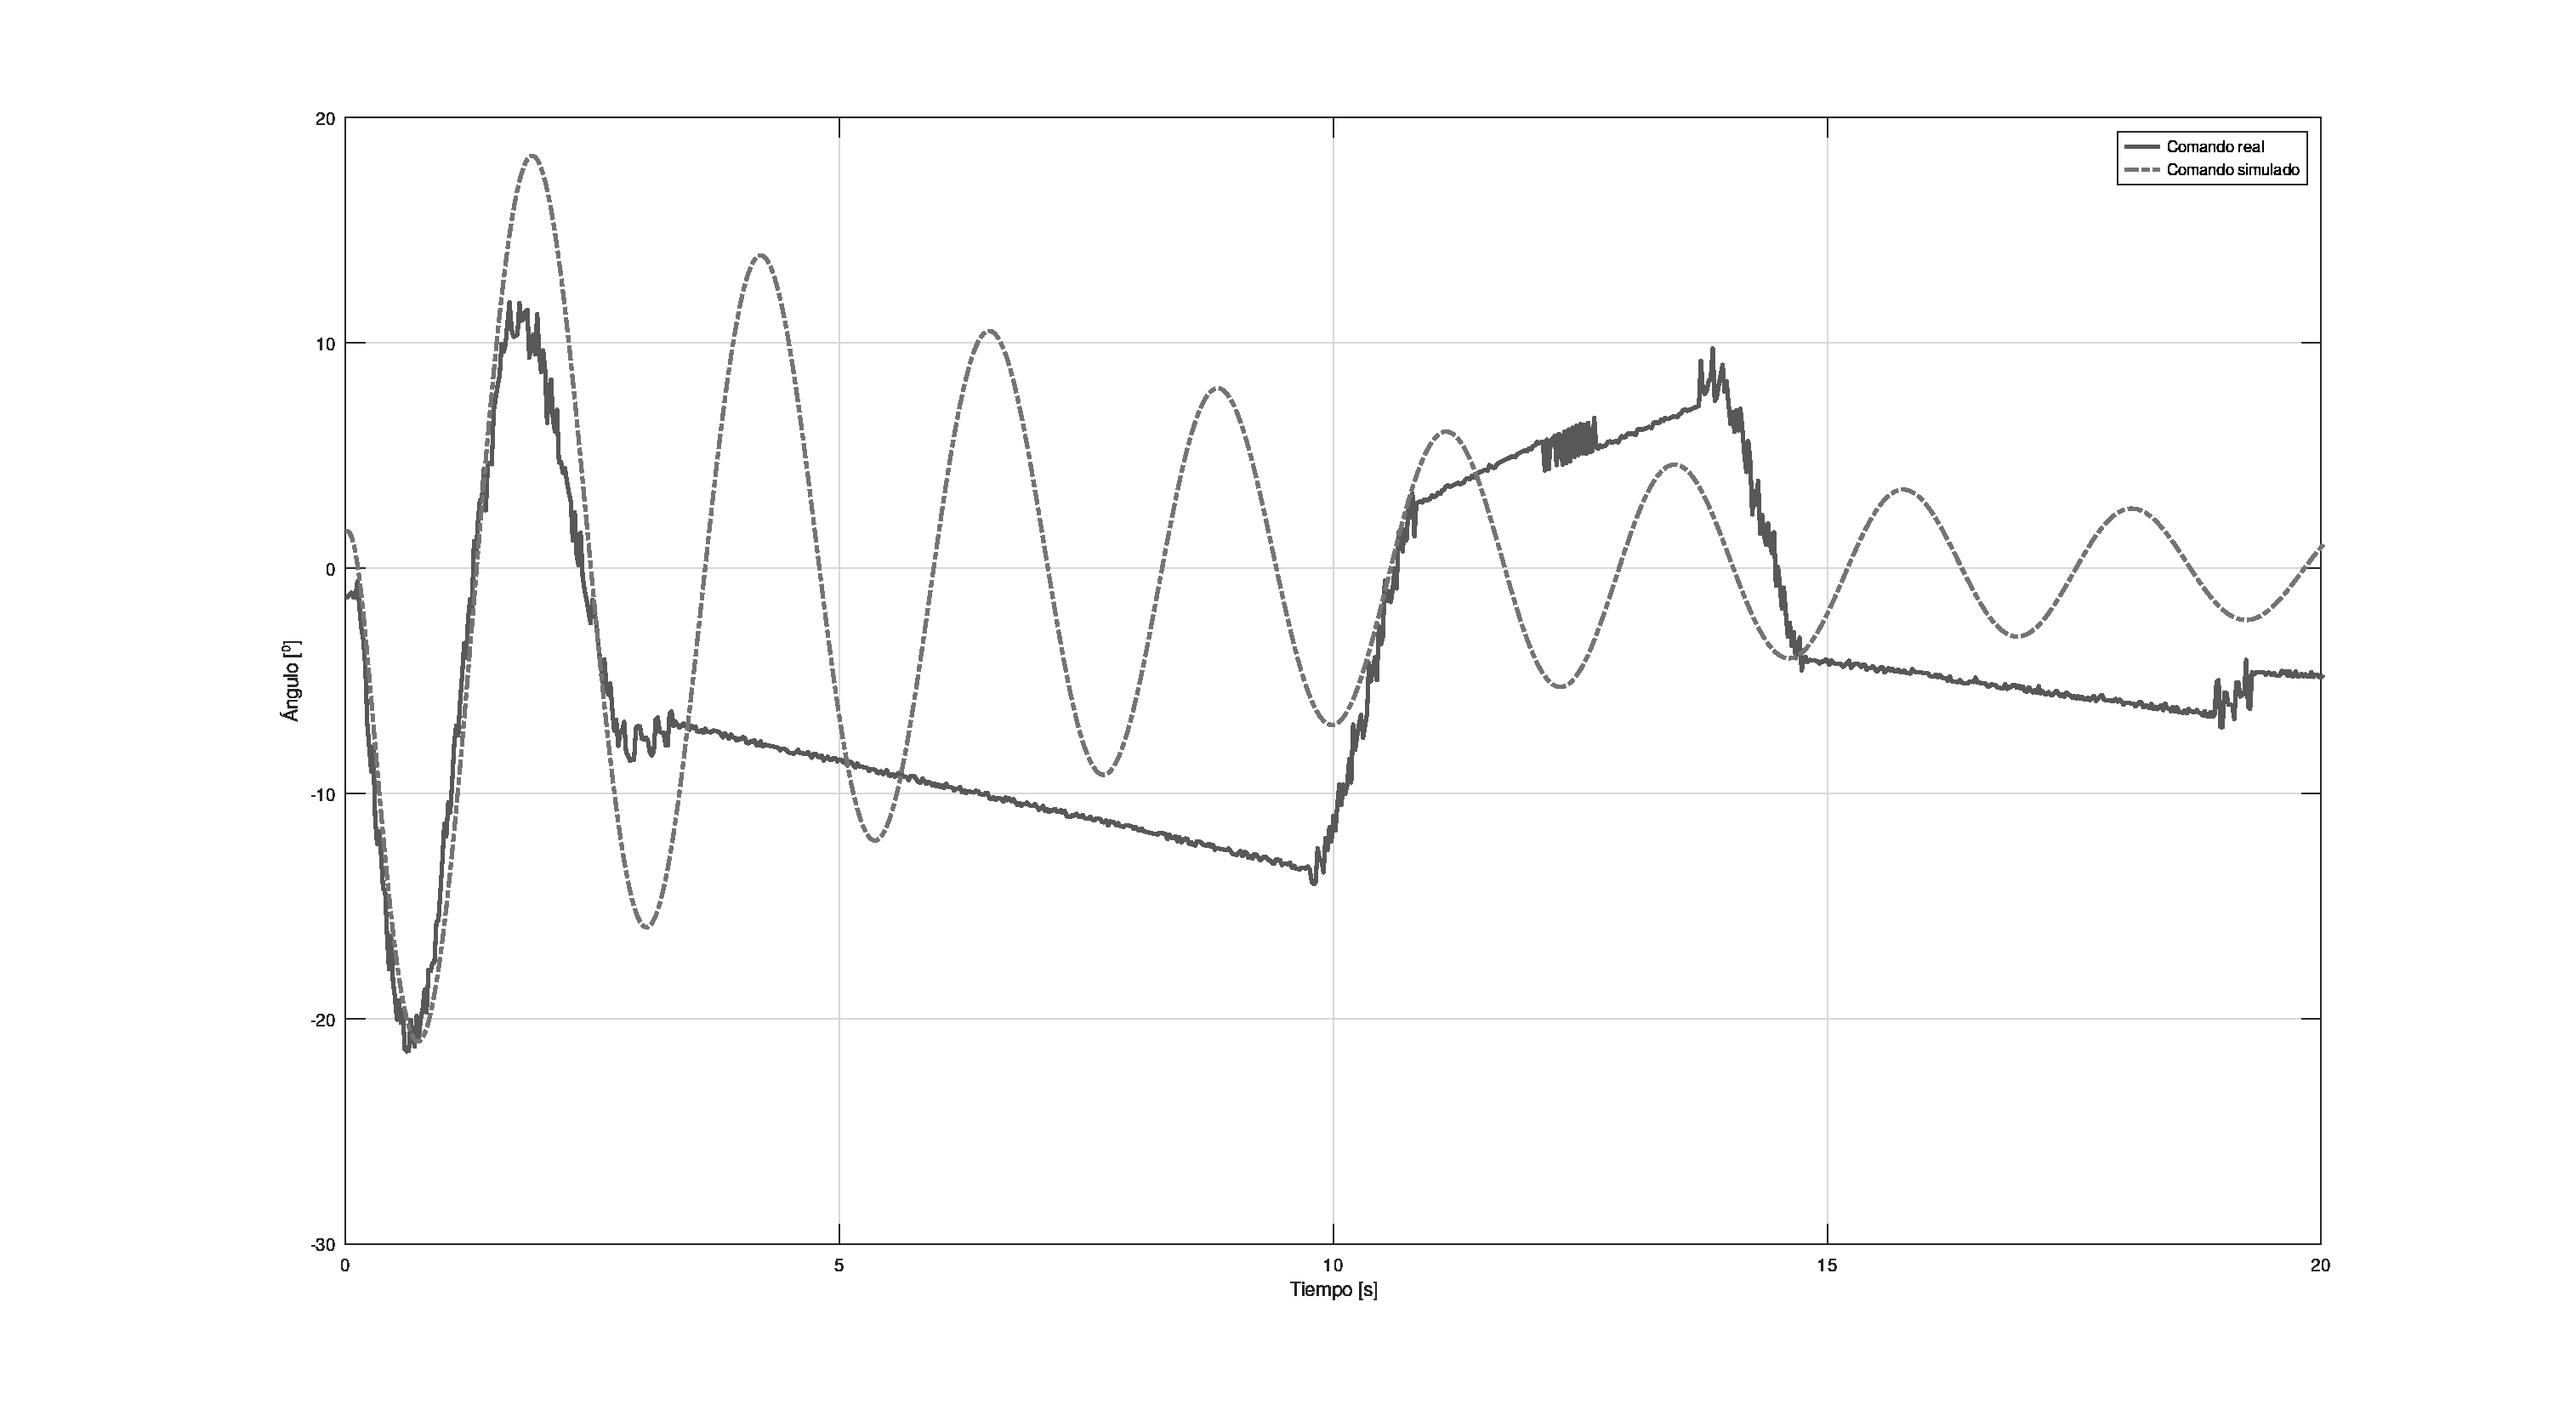
\includegraphics[width=\linewidth]{img/pi-pert-cont.eps}
    \caption{Acción de control del sistema real y simulado ante una perturbación tipo impulso, y un lazo cerrado con un controlador tipo PI.}
    \label{fig:pi-pert-cont}
\end{figure}

% vim: ts=4 sts=4 sw=4 et lbr
